 
% Kelompok Penentuan Waktu
% Muhammad Nur Ikhsan (1154087)
% Wahyu Maruti Adjie (1154034)
% Ilman Mubarik 	(1154114)
% Emy Safitri		(1154102)
% Andi Ikram Maulana	(1154065)

\section{Sejarah Waktu}

Sejarah Penentuan Waktu diurutkan secara kronologis dalam tabel skala waktu geologi 
yang dibagi menjadi beberapa interval sesuai analisis stratigrafi. 
Ada 4 garis waktu yang ada, garis waktu yang pertama menunjukkan waktu dari masa terbentuknya Bumi sampai waktu sekarang\cite{suryasejarah}.  Skala waktu kedua menunjukkan eon terbaru dengan skala yang diperluas. Skala waktu kedua, ketiga, dan keempat merupakan sub bagian dari skala waktu sebelumnya yang ditunjukkan oleh tanda bintang. 
Alasan lain untuk memperluas skala waktu adalah HOLOSEN (jangka waktu) terakhir terlalu kecil untuk dapat ditampilkan dengan jelas
pada skala waktu ketiga disebelah kanan. Gambar \ref{sejarahpenentuan} adalah ilustrasi skala waktu.

\begin{figure}[ht]
\centerline{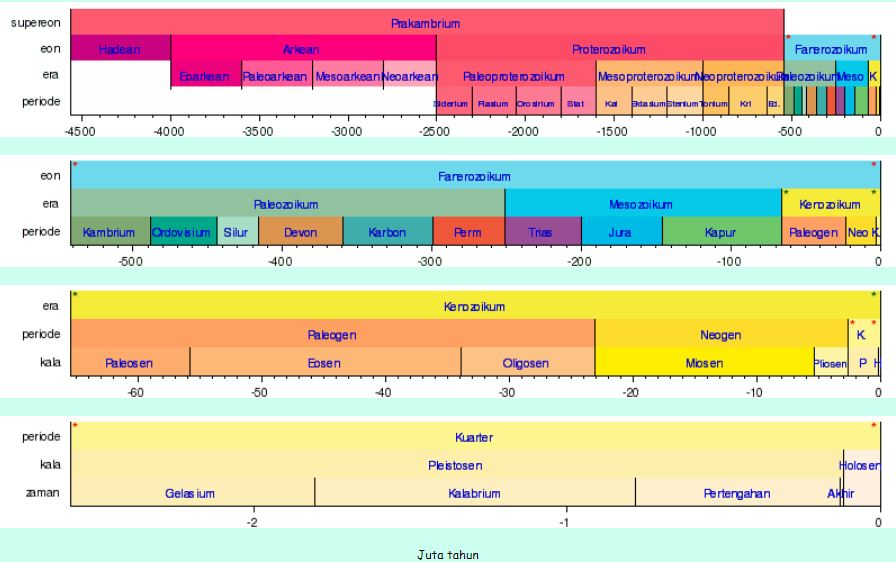
\includegraphics[width=1\textwidth]{figures/sejarahpenentuan.JPG}}
\caption{Gambar skala waktu yang ditetapkan.}
\label{sejarahpenentuan}
\end{figure}

\section{Penentuan Waktu}
Pada pembahasan diatas, kita telah membahas tentang sejarah waktu, dan skala waktu. 
Dari penjelasan tersebut, maka dibuatlah suatu pergerakan rotasi bumi. 
Gerakan ini disebut gerakan semu Matahari yang digunakan dalam penentuan waktu (jam).

\subsection{Hari Matahari}
 Menurut artikel dari rachman planet mengemukakan bahwa satu hari matahari ditentukan
 oleh selang waktu antara dua kulminasi \cite{rachmanplanet}. Kulminasi Atas disebut tengah hari (pukul 12.00)
 dan Kulminasi Bawah adalah saat tengah malam (pukul 24.00 atau pukul 00.00). 
 Dalam kegiatan kita sehari-hari, satu hari matahari adalah waktu yang diperlukan
 Matahari bergerak semu mengelilingi Bumi, terhitung mulai titik Kulminasi Atasnya
 hingga kembali lagi ke titik Kulminasi Atasnya lagi. Dari hasil pengamatan Simamora, ternyata 
 panjang hari matahari (semu) selama setahun berbeda-beda(tidak konstan), 
 hal ini disebabkan:
 \begin{enumerate}
 \item Bentuk lintasan revolusi Bumi adalah elips.
 Dalam perputaran Bumi mengelilingi Matahari membuat lintasan berbentuk elips 
 sehingga waktu lintasan mengelilingi Matahari (perihelium) 
 pergerakannya cepat dan pada waktu lintasan terjauh 
 dengan Matahari (aphelium) pergeseran nya pada ekliptika lambat. 
 Dengan adanya kecepatan gerak Bumi mengelilingi matahari (revolusi)
 tidak sama dengan rotasi bumi tetap, maka terjadilah pergeseran semu
 pada ekliptika tidak seragam, akibatnya saat Matahari mencapai 
 kulminasi nya tidak sama. Artinya panjang hari pada hari matahari 
 setiap harinya tidak sama.
 
 \item	Inklinasi ekliptika pada ekuator langit.
 Oleh sebab perputaran Bumi pada sumbu nya (rotasi) miring maka kedudukan
 bidang ekuator langit dengan bidang ekliptika membentuk sudut 23,50 .
 Akibat dari rotasi bumi itu, sepanjang tahun Matahari seolah-olah bergeser ke arah
 Utara atau ke arah Selatan. Enam bulan berada di belahan Utara dan 
 enam bulan di belahan bumi Selatan. Gerakan tersebut menyebabkan 
 terjadi perbedaan panjang hari terutama pada lintang geografis sedang
 atau tinggi, baik di belahan Bumi Utara atau belahan Bumi Selatan.
 \end{enumerate}
\subsection{Hari Bintang}

Hari Bintang adalah selang waktu yang diperlukan sebuah Bintang untuk berkombinasi 

 pada tempat yang sama pada saat berikutnya dalam meridian langit yang 
 sama dari suatu tempat. Satu hari bintang (sehari semalam bintang) adalah 
 waktu yang diperlukan sebuah bintang (lebih umum disebut titik Aries) bergerak semu
 mengelilingi Bumi mulai dari titik Kulminasi Atasnya sampai ke titik Kulminasi Atasnya 
 lagi. Hari Matahari lamanya 24 jam sedangkan hari Bintang adalah 23 jam 56 menit. 
 Jadi perbedaan antara hari Matahari dan  hari Bintang adalah 1/365 x 24 jam atau 
 1/365 x 1440 menit yaitu 3 menit 56 detik di bulatkan menjadi 4 menit. 
 Jadi pada hari berikutnya Bintang tersebut akan berkulminasi 4 menit lebih awal.
 Anda dapat menghitung selama 30 hari menjadi 30 $\times$ 4 menit yaitu 120 menit atau 2 jam. 

Jadi setelah 12 bulan (1 tahun) yaitu  12 $\times$ 2 jam = 24 jam. Dengan demikian setahun
 kemudian baru Bintang tersebut akan berkulminasi pada jam yang sama. 
 Jadi seolah-olah langit perbintangan berputar kurang lebih 10 setiap hari. 
 Satu tahun Bintang 3600 dibagi 365,25 hari Matahari.

Sebagai contoh, pada tanggal 23 Maret Bintang Regulus berkulminasi pada pukul 08.00,
 pada tanggal 23 April bintang tersebut berkulminasi pukul 06.00, dan pada tanggal 23 Mei 
 Bintang tersebut berkulminasi pukul 04.00. Dari pendataan tersebut maka: 
\begin{itemize}
 \item 1 hari bintang = 1 hari matahari dikurangi 4 menit, 
 \item 1 jam bintang = 1 jam matahari dikurangi 1 detik. 
\end{itemize}
 Dari perhitungan yang dijelaskan maka ada tanggal-tanggal istimewa 
 untuk waktu Bintang dan waktu Matahari, yaitu:
 \begin{itemize}
	\item Tanggal 21 Maret, pukul 00.00 waktu Bintang = pukul 12.00 waktu Matahari,
	\item Tanggal 21 Juni, pukul 00.00 waktu Bintang = pukul 06.00 waktu Matahari,
	\item Tanggal 23 September, pukul 00.00 waktu Bintang = pukul 00.00 waktu Matahari
	\item Tanggal 22 Desember, pukul 00.00 waktu Bintang = pukul 18.00 waktu Matahari.
\end{itemize}
	

 Jadi hubungan antara Lokal Siderial Times (LST) atau waktu Bintang, 
 dengan Local Civil Times (LCT) dan jumlah hari perbedaan sejak 22,7 September 
 (dibulatkan 23 September) sampai tanggal yang ditentukan adalah:
 LST = LCT + ($\frac${4.69}{70}) D. Catatan: $\frac${4.69}{70} = 4 $\times$ $\frac${69}{70} = 3 menit 56 Detik.	
 
\subsection{Hari Matahari Menengah/Matahari Khayal dan Perata Waktu}
 Dari penjelasan diatas kita, dapat mengetahui bahwa Matahari bukanlah penunjuk 
 waktu yang sangat tepat. Oleh sebab itu, untuk keperluan pembagian waktu yang tepat
 yang kita gunakan sehari-hari, para ahli pun mendasarkan perhitungannya pada Matahari
 khayal. Matahari khayal ini adalah Matahari yang dianggap atau dimisalkan ada, 

 yang kecepatan pergeseran nya hampir serupa dengan pergeseran Matahari sebenarnya.
 
Perbedaannya adalah Matahari khayal ini bergeser sepanjang ekuator langit 
 dengan kecepatan pergeseran yang tetap (konstan) atau seragam, sehingga panjang satu
 “hari matahari khayal” = panjang rata-rata “hari matahari sebenarnya”. 
 Oleh karena itulah hari matahari khayal disebut pula hari matahari menengah.

 
  Pada saat matahari menengah inilah didasarkan pembagian waktu pada jam yang kita gunakan sehari-hari, karena setiap hari matahari menengah panjangnya tetap sama sepanjang tahun.

	1 hari matahari menengah = 24 jam waktu matahari menengah 
	1 jam waktu matahari menengah = 60 menit waktu matahari menengah
	1 menit waktu matahari menegah = 60 detik waktu matahari menengah
	
	Bandingkan
	1 hari matahari menengah = 24 jam waktu matahari menengah (jam kita)
							 = 24 jam 4 menit waktu bintang (24 jam 3menit 57detik)
	1 hari bintang		     = 24 jam waktu bintang
							 = 23 jam 6menit waktu matahari menengah 

							  (tepat nya 23 jam 56 menit 4 detik)}
								  
Waktu matahari menengah dimulai ketika matahari menengah berada pada titik
 Kulminasi bawahnya (pukul 00.00 waktu matahari menengah), cara membedakannya mulai 

 dari waktu bintang yang dimulai pada saat titik Aries berada
 pada titik Kulminasi Atasnya (pukul 00.00 waktu bintang).


Hari Matahari Menengah kadang-kadang lebih sedikit pendek dari Hari Matahari 
 Sebenarnya tetapi terkadang lebih panjang.   Perbedaan maksimal hanyalah 
 sampai kira-kira seperempat jam. Perbedaan waktu ini disebut Perata Waktu, 
 dengan rumus:
				Perata Waktu = Hari Matahari Menengah-Hari Matahari Sebenarnya

							(Simamora,P., 1975: 72)

								
Perata waktu ini dinyatakan dengan tanda positif (+) jika 
 matahari menengah mendahului matahari sebenarnya dan tanda negatif (-)
 jika terjadi sebaliknya. Perata waktu terbesar terjadi pada 11 Februari,
 yaitu + 14 menit dan 2 November, yaitu – 16 menit. Dalam satu tahun terjadi 
 empat kali panjang hari matahari menengah sama dengan pajang hari matahari sebenarnya,
 yaitu 15 April, 14 Juni, 1 September, dan 24 Desember. Pada hari-hari ini perata 
 waktunya adalah 0 menit. Untuk lebih jelasnya perhatikan gambar \ref{sejarahwaktu_Capture}.								
	
	\begin{figure}[ht]
	\centerline{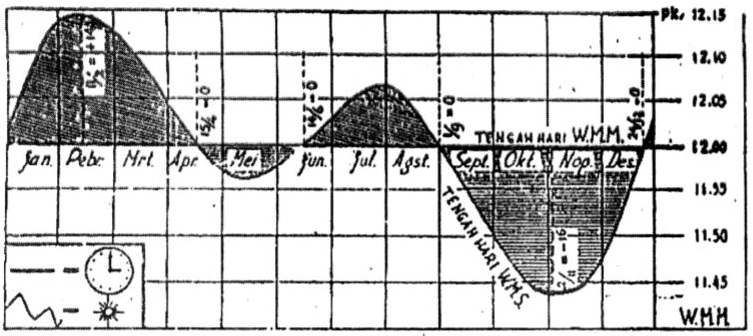
\includegraphics[width=1\textwidth]{figures/sejarahwaktu_peratawaktu}}
	\caption{Perata Waktu}
	\label{sejarahwaktu_Capture}
	\end{figure}

 Dari gambar \ref{sejarahwaktu_Capture} kita dapat mengetahui pula bahwa sekitar bulan Januari, Februari
 Maret, Juli, dan Agustus matahari sebenarnya lebih lambat sampai titik Kulminasi atasnya,
 sehingga sore lebih lama terangnya.
 
	Contoh: Pada tanggal 2 November jam di tangan kita (waktu matahari menengah) 
	menunjukkan pukul 12.00, tetapi Matahari di langit masih belum tiba di titik Kulminasi 
	Atasnya, baru -16 menit kemudian hal itu terjadi, yaitu pada pukul 11.44 waktu matahari 
	menengah. Sebaliknya, pada bulan Oktober, November, dan Desember matahari menengah 
	lebih lambat daripada matahari sebenarnya. Pagi hari Matahari telah terbit sedangkan 
	jam kita masih menunjukkan kurang dari pukul 06.00. Pada sore harinya pukul 06.00 sudah
	gelap. Hal ini terjadi pada sekitar khatulistiwa (termasuk di Indonesia), 
	di daerah-daerah sedang dan kutub tentunya berbeda.
	

\subsection{Greenwich Mean Time(GMT)}
Greenwich Mean Time (GMT) adalah tempat yang menjadi

 patokan waktu dunia berada. Jika ditentukan dengan penentuan waktu GMT lebih mudah kita
 dapat menghitung waktu-waktu di seluruh permukaan Bumi. Bagi daerah yang
 berada di belahan barat (meridian barat) waktu setempat adalah waktu GMT
 ditambah dengan hasil kali perbedaan meridian dengan 4 menit sedangkan daerah
 yang berada di belahan timur (meridian timur) waktu setempat adalah waktu GMT
 dikurangi dengan hasil kali antara selisih meridian dengan 4menit. 
 cara perumusannya dengan menggunakan:
					LMT = GMT +(M $\cdot$ 4)
			(Dardjosoemartp, dkk.,1991: 445)
\begin{itemize}		
\item LMT  = Local Mean Time / Waktu Setempat 
\item GMT  = Greenwich Mean Time / waktu GMT
\item +	 = + bila di BB dan – bila di BT 
\item (M.4) = meridian (bujur) x 4 menit
\end{itemize}

\section{Waktu Standar}
Tempat-tempat yang terletak pada garis meridian yang sama, mempunyai waktu yang sama.
 Jika demikian, seluruh permukaan Bumi terdapat 360 waktu yang bedanya 4 menit.

 Hal ini tentu rumit dalam kehidupan sehari-hari. Oleh sebab itu, disepakatilah untuk
 membagi permukaan Bumi atas 24 daerah waktu saja yang disebut waktu standar.
 
 Waktu standar disebut juga Zone Time, yaitu waktu yang ditetapkan setiap 
 selisih 150 adalah 60 menit (1 jam) dengan lingkup daerah yang berada pada 00 – 150
 atau 150 – 300, dan seterusnya baik di Bujur Timur maupun Bujur Barat.

 Kongres Internasional memutuskan tentang garis-garis meridian (International Meridian Conferense) 
 di Washington menetapkan waktu standar dunia yang dibagi menjadi 24 daerah berdasarkan
 perbedaan meridian 150 . Setiap daerah mempunyai selisih waktu 1 jam.
 Akan tetapi berdasarkan pembagian wilayah ke pemerintahan atau kontinen (pulau/benua)
 maka ada sedikit pergeseran. Batas yang terdapat pada 1800 BT dan 1800 BB berupa garis
 yang berkelok-kelok. Perhatikan gambar \ref{sejarahwaktu_Capture1} di bawah ini:
 
 \begin{figure}[ht]
 \centerline{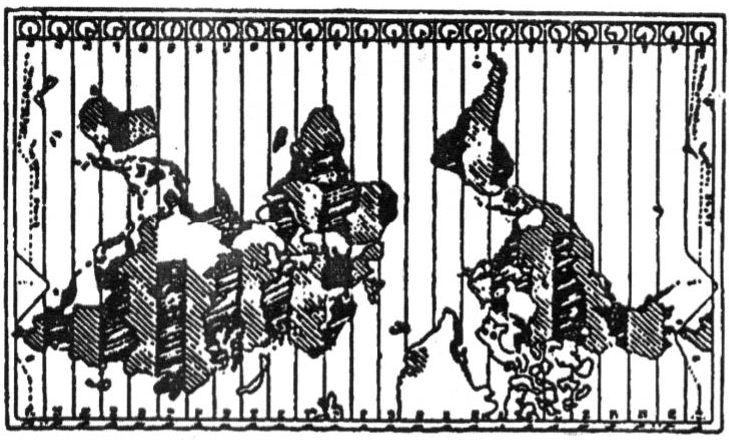
\includegraphics[width=1\textwidth]{figures/sejarahwaktu_dunia}}
 \caption{Pembagian Daerah Waktu di Dunia.}
 \label{sejarahwaktu_Capture1}
 \end{figure}
 

 
Setiap negara mempunyai pembagian daerah waktu yang berbeda-beda karena letak pada meridianya berbeda. 
 Indonesia terletak antara 950 BT – 1410 BT. Oleh karena Indonesia mempunyai rentang meridian 1410 – 950 = 460 , 
 maka Indonesia di bagi menjadi 3 daerah waktu, yakni Waktu Indonesia bagian Barat (WIB),
 Indonesia bagian Tengah (WITA), dan Waktu Indonesia bagian Timur (WIT) dengan selisih
 satu jam. Untuk lebih jelasnya, perhatikan gambar \ref{sejarahwaktu_Capture2}.

 
 \begin{figure}[ht]
 \centerline{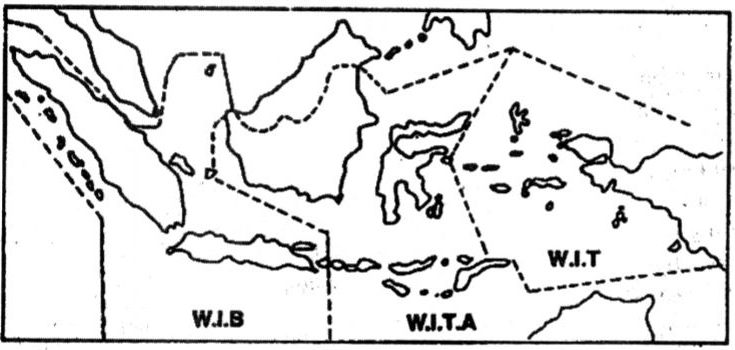
\includegraphics[width=1\textwidth]{figures/sejarahwaktu_indo64}}
 \caption{Pembagian Waktu di Indonesia Tahun 1964}
 \label{sejarahwaktu_Capture2}
 \end{figure}
 


Indonesia mempunyai tiga meridian standar, yaitu meridian 1050 BT untuk daerah WIB, 
 1200 BT untuk daerah WITA, dan 1350 untuk WIT. Dengan demikian waktu lokal nya (LMT) 

 masing-masing adalah waktu Greenwich 
 ditambah $\frac${105}{15} untuk WIB, $\frac${120}{15} untuk WITA, dan $\frac${135}{15} untuk WIT .
 Jika waktu GMT pukul 12.00, maka: WIB = 12.00 + ($\frac${105}{15}=7) yaitu pukul 19.00,
 WITA = 12.00 + ($\frac${120}{15}= 8) yaitu pukul 20.00, 

 dan WIT = 12.00 + ($\frac${135}{15}=9) yaitu pukul 21.00(Hidayat,B.,1978: 42).
